% !TeX root = ../../main.tex

Do przeprowadzenia eksperymentów użyto dwóch zbiorów danych, w skład których wchodzą między innymi zdjęcia otrzymane od firmy \blue{}.
Jeden zbiór, zwany dalej zbiorem \textit{high} pochodzi z kamer ustawianych ponad kortem.
Drugi zbiór, zwany dalej zbiorem \textit{low}, pochodzi z kamer sytuowanych na podłodze, tuż przy liniach kortu.


\begin{figure}[!htb]
  \minipage{0.45\textwidth}
    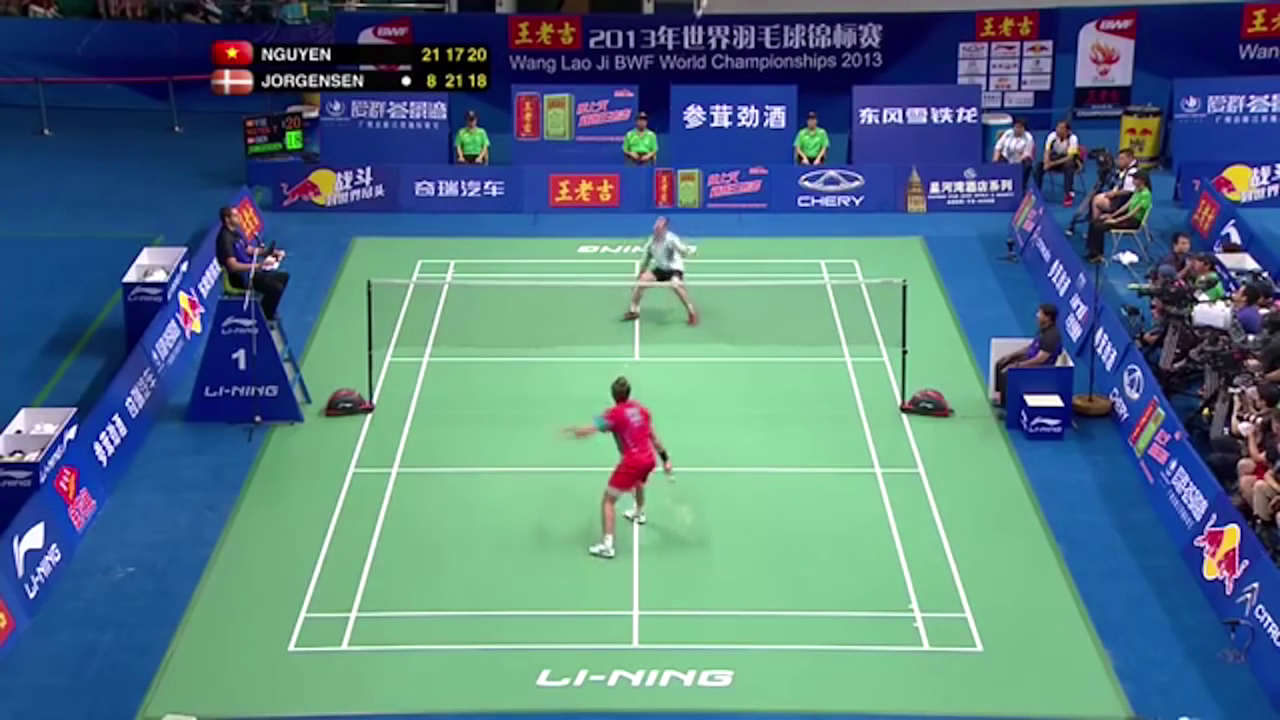
\includegraphics[width=\linewidth]{../../badminton/datasets/high/split/test_court2-00002.png}
    \caption{Przykładowy obraz ze zbioru danych \textit{high}}
  \endminipage\hfill
  \minipage{0.45\textwidth}
    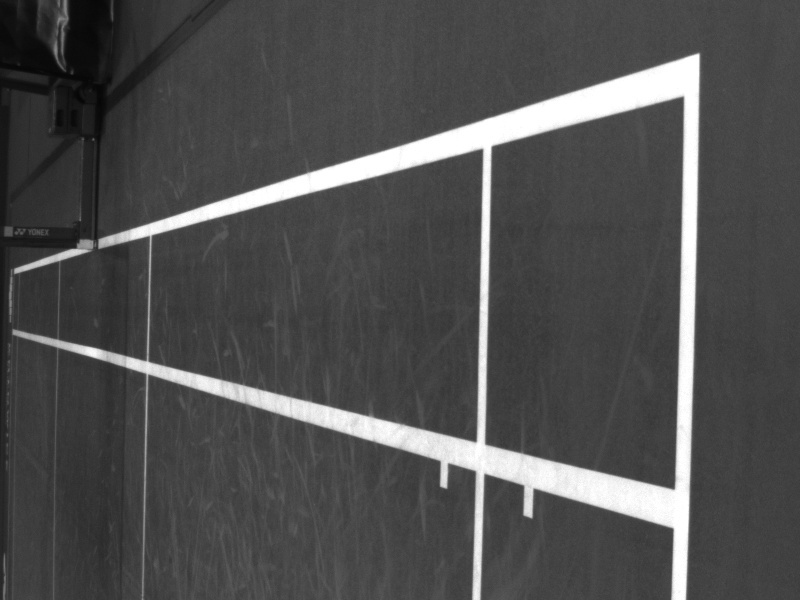
\includegraphics[width=\linewidth]{../../badminton/datasets/low/split/1564909032792410075.jpg}
    \caption{Przykładowy obraz ze zbioru danych \textit{low}}
  \endminipage\hfill
\end{figure}

Zbiór \textit{low} zawiera obrazy pozyskane wyłącznie od firmy \blue{}, o rozdzielczości 896x640 pikseli.

\begin{table}[!h]
	\centering
	\caption{Liczność zbiorów danych}
	\vspace{6pt}
	{\footnotesize
		\begin{tabular}{|c|c|c|c|}
			\hline \textbackslash & Liczność \\
      \hline Zbiór \textit{high} & 97 \\
      \hline Zbiór \textit{low} & 207 \\
      \hline
		\end{tabular}
	}
	\vspace{0pt}
\end{table}

Zbiór danych \textit{high} składa się z 36 obrazów o wymiarach 1280x720 pikseli, 6 obrazów o rozdzielczości 480x360, 4 obrazów o rozdzielczości 640x480, i pozostałych obrazów o różnych rozdzielczościach, od 259x194 pikseli do 2040x1530 pikseli. Obrazy pochodzą z różnych źródeł - od firmy \blue{}, z Internetu oraz ze zrzutów ekranu transmisji zawodów sportowych.
